\section{逐轮自归因分解}
\label{sec:appendix:self-attribution}

本附录在 \S\ref{sec:experiments:rq3b} 的汇总自归因结果基础上加以扩展，给出在“修复/回归 $\times$ 精确率/召回率”四个面板上的逐轮分解。

\Cref{fig:pred-fix,fig:pred-reg} 展示了在“修复/回归 $\times$ 精确率/召回率”四个面板上的逐轮分解。柱状图把每个分母（精确率对应预测数、召回率对应实际数）分解为深蓝色的 TP 与浅色的 FP 或 FN；虚线在右侧 $0$ 到 $100\%$ 的坐标轴上刻画该指标，实线则显示同期的 pass@1。修复精确率与修复召回率在各轮之间都从接近零一路摆动到接近饱和，因此演化模型对自身改进的因果归因虽有噪声，但仍是有信息量的。相比之下，回归预测始终贴近下界，在大多数轮次中低于 $25\%$：在这 9 轮中，智能体共发出 43 条不重复的回归预测，其中只有 5 条命中，累计 $P=11.6\%$；与此同时，有 40 次回归是智能体未曾预见却实际发生的，累计 $R=11.1\%$。

\begin{figure}[t]
    \centering
    \begin{minipage}{0.49\linewidth}
        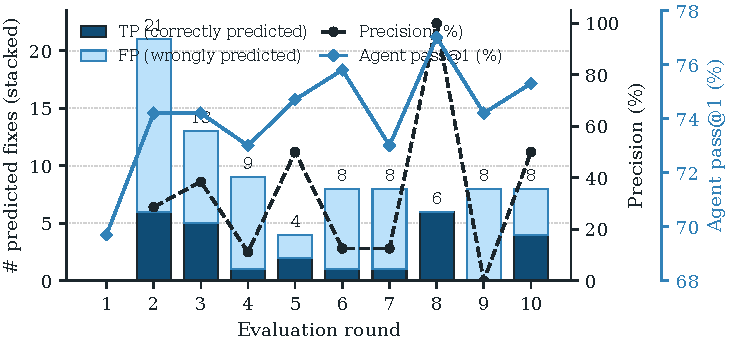
\includegraphics[width=\linewidth]{figures/prediction_fix_precision.pdf}
    \end{minipage}
    \hfill
    \begin{minipage}{0.49\linewidth}
        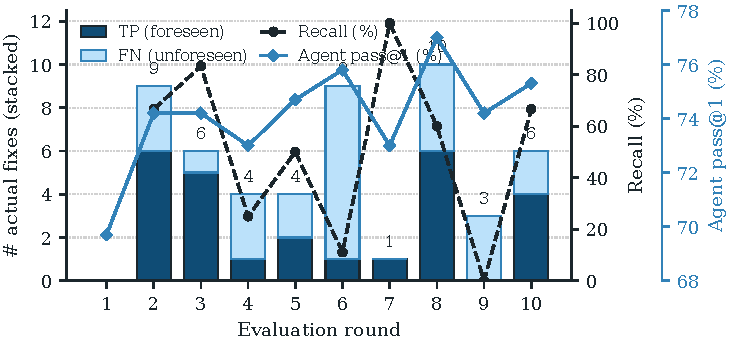
\includegraphics[width=\linewidth]{figures/prediction_fix_recall.pdf}
    \end{minipage}
    \caption{逐轮修复预测。左：精确率。右：召回率。柱状图把每个分母分解为 TP 与 FP 或 FN；折线叠加显示该指标与同期的 pass@1。}
    \label{fig:pred-fix}
\end{figure}

\begin{figure}[t]
    \centering
    \begin{minipage}{0.49\linewidth}
        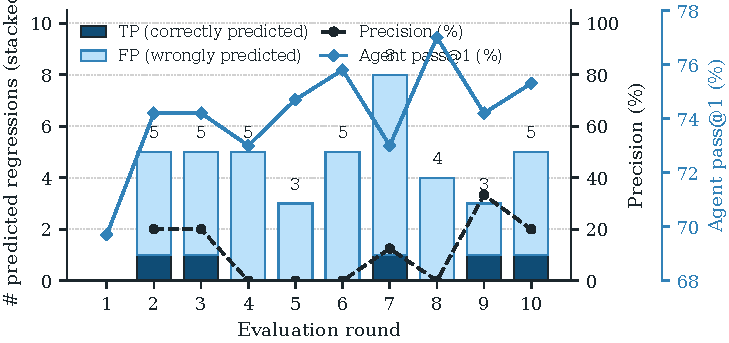
\includegraphics[width=\linewidth]{figures/prediction_regression_precision.pdf}
    \end{minipage}
    \hfill
    \begin{minipage}{0.49\linewidth}
        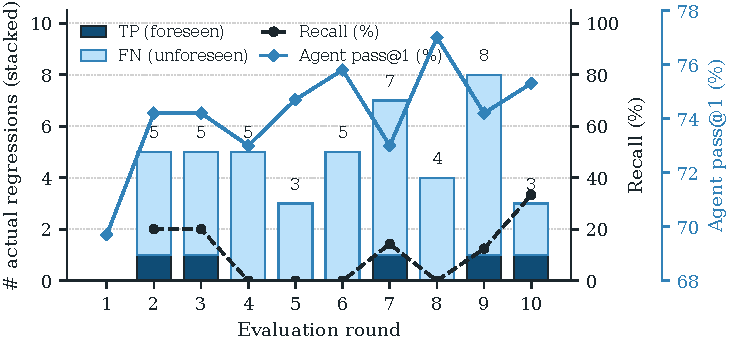
\includegraphics[width=\linewidth]{figures/prediction_regression_recall.pdf}
    \end{minipage}
    \caption{逐轮回归预测。左：精确率。右：召回率。编码方式与图~\ref{fig:pred-fix} 相同。}
    \label{fig:pred-reg}
\end{figure}
